%%%%%%%%%%%%%%%%%%%%%%% file template.tex %%%%%%%%%%%%%%%%%%%%%%%%%
%
% This is a general template file for the LaTeX package SVJour3
% for Springer journals.          Springer Heidelberg 2010/09/16
%
% Copy it to a new file with a new name and use it as the basis
% for your article. Delete % signs as needed.
%
% This template includes a few options for different layouts and
% content for various journals. Please consult a previous issue of
% your journal as needed.
%
%%%%%%%%%%%%%%%%%%%%%%%%%%%%%%%%%%%%%%%%%%%%%%%%%%%%%%%%%%%%%%%%%%%
%
% First comes an example EPS file -- just ignore it and
% proceed on the \documentclass line
% your LaTeX will extract the file if required
\begin{filecontents*}{example.eps}
%!PS-Adobe-3.0 EPSF-3.0
%%BoundingBox: 19 19 221 221
%%CreationDate: Mon Sep 29 1997
%%Creator: programmed by hand (JK)
%%EndComments
gsave
newpath
  20 20 moveto
  20 220 lineto
  220 220 lineto
  220 20 lineto
closepath
2 setlinewidth
gsave
  .4 setgray fill
grestore
stroke
grestore
\end{filecontents*}
%
\RequirePackage{fix-cm}
%
%\documentclass{svjour3}                     % onecolumn (standard format)
%\documentclass[smallcondensed]{svjour3}     % onecolumn (ditto)
\documentclass[smallextended]{svjour3}       % onecolumn (second format)
%\documentclass[twocolumn]{svjour3}          % twocolumn
%
\smartqed  % flush right qed marks, e.g. at end of proof
%
\usepackage{graphicx}
\usepackage{listings}
%
% \usepackage{mathptmx}      % use Times fonts if available on your TeX system
%
% insert here the call for the packages your document requires
%\usepackage{latexsym}
% etc.
%
% please place your own definitions here and don't use \def but
% \newcommand{}{}
%
% Insert the name of "your journal" with
% \journalname{myjournal}
%
\begin{document}

\title{Requirements and design criteria for a Linked Open Statistical Data API
%\thanks{Grants or other notes
%about the article that should go on the front page should be
%placed here. General acknowledgments should be placed at the end of the article.}
}
\subtitle{Do you have a subtitle?\\ If so, write it here}

%\titlerunning{Short form of title}        % if too long for running head

\author{First Author         \and
        Second Author %etc.
}

%\authorrunning{Short form of author list} % if too long for running head

\institute{F. Author \at
              first address \\
              Tel.: +123-45-678910\\
              Fax: +123-45-678910\\
              \email{fauthor@example.com}           %  \\
%             \emph{Present address:} of F. Author  %  if needed
           \and
           S. Author \at
              second address
}

\date{Received: date / Accepted: date}
% The correct dates will be entered by the editor


\maketitle

\begin{abstract}
Insert your abstract here. Include keywords, PACS and mathematical
subject classification numbers as needed.
\keywords{First keyword \and Second keyword \and More}
% \PACS{PACS code1 \and PACS code2 \and more}
% \subclass{MSC code1 \and MSC code2 \and more}
\end{abstract}

\section{Introduction}\label{sec:intro}


Motivation:
\begin{itemize}
\item  Linked Open Statistical Data (LOSD)
\item Need to facilitate LSD re-use without the need to know QB vocabulary, RDF etc and easily build apps that consume JSON on top of LOSD
\item Re-use s/w tools across LOSD datasets 
\end{itemize}

\textbf{Objective: To specify the requirements of an API that standardizes the interaction, including input and output, with LOSD.}

\section{Methodology}\label{sec:methodology}

Related work:
\begin{itemize}
\item  OLAP APIs – interaction with multidimensional data (input): Oracle OLAP API [1], Olap4j [2], ++
\item Standardization of outcome: Json-stat, Json-ld, ++
\end{itemize}

Discussion with developers: Workshop, +++

\section{Solution overview}\label{sec:overview}



\begin{figure}
  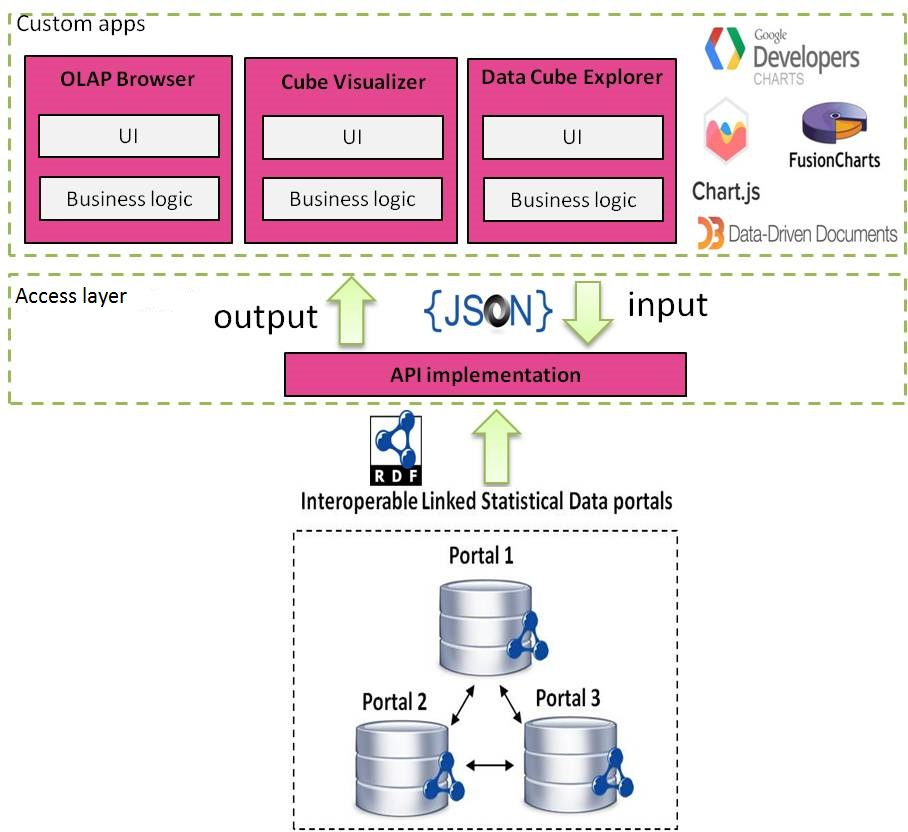
\includegraphics{images/overview.jpg}
\caption{Solution overview}
\label{fig:overview}
\end{figure}


\section{Requirements and design criteria}\label{sec:reqs}

\begin{itemize}
\item need to know what datasets are available
\item need to know about structure to subset the observations
\item in order not to return everything, need to subset
\item don't necessarily need a n-array/ tabular response - array of observations is sufficient. can always get back to the table
\item Filtering
\item Multilinguality
\item Ordering \& paging
\item merging, aggregations
\item json-ld representation is sufficient for query and response format
\item ++
\end{itemize}

API functionality:
\begin{itemize}
\item GET dataset-metadata
\item GET dimensions
\item GET attributes
\item GET measures
\item GET dimension-values
\item GET attribute-values
\item GET dimension-levels
\item GET slice
\item GET table
\item GET cubes
\item GET aggregationSetcubes
\item GET create-aggregations
\item GET cubeOfAggregationSet
\end{itemize}

\cite{Janssen:2012}

possible example for slice/ observation-selection query:
\begin{verbatim} 
{ 
  "jqql:dataset": "scot:home-care-clients",
  "jqql:filter": {
"dimension:gender": "gender:male",
   "dimension:age": { "jqql:greater-than": 50 }
  },
  "jqql:order": {
    "dimension:refPeriod": { "jqql:order-predicate": "ui:sortPriority", "jqql:direction": "jqql:asc"}
  },
  "jqql:page": {
    "jqql:limit": 10,
    "jqql:offset": 0
  }
}
\end{verbatim}

output:
\begin{verbatim} 
{ "observations": [ 
	{ "Average Cost": "1182", 
   	  "Date": "1-1-2013", 
	  "Day": "Tuesday", 
	  "Number of crashes": "5",
	  "Time": "No available time",
      "Total Cost": "5908", 
	  "@id": http://id.mkm.ee/observation/1" }, 
	{ "Average Cost": "400",
	  "Date": "1-1-2013",
	  "Day": "Tuesday",
	  "Number of crashes": "1",
	  "Time": "24:00",
 	  "Total Cost": "400",
	  "@id": "http://id.mkm.ee/observation/2" }
]}
\end{verbatim}

\section{Implementation}\label{sec:impl}

\section{Conclusion}\label{sec:conclusion}


%
% For tables use
\begin{table}
% table caption is above the table
\caption{Please write your table caption here}
\label{tab:1}       % Give a unique label
% For LaTeX tables use
\begin{tabular}{lll}
\hline\noalign{\smallskip}
first & second & third  \\
\noalign{\smallskip}\hline\noalign{\smallskip}
number & number & number \\
number & number & number \\
\noalign{\smallskip}\hline
\end{tabular}
\end{table}


%\begin{acknowledgements}
%If you'd like to thank anyone, place your comments here
%and remove the percent signs.
%\end{acknowledgements}

% BibTeX users please use one of
\bibliographystyle{spbasic}      % basic style, author-year citations
%\bibliographystyle{spmpsci}      % mathematics and physical sciences
%\bibliographystyle{spphys}       % APS-like style for physics
\bibliography{qbbibfile}   % name your BibTeX data base


\end{document}


